\documentclass[tikz,border=3mm]{standalone}
\usepackage[utf8]{inputenc}
\usepackage[T1]{fontenc}
\usepackage{helvet}
\renewcommand{\familydefault}{\sfdefault}
\usetikzlibrary{arrows.meta,positioning}
\begin{document}

\tikzset{every node/.append style={font=\sffamily\small}}
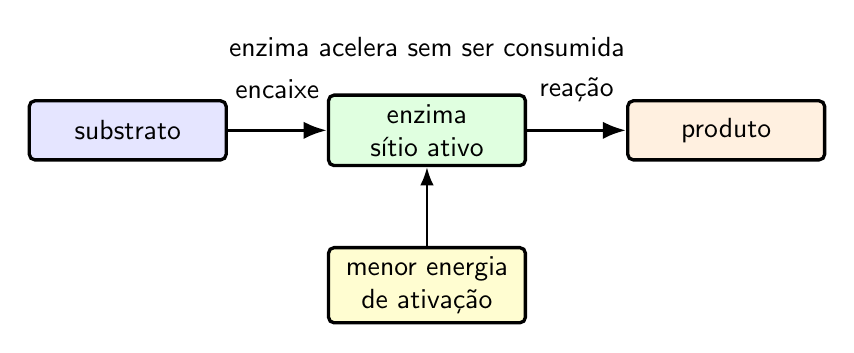
\begin{tikzpicture}[>=Latex,node distance=0.8cm]
  \tikzstyle{box}=[draw,rounded corners=2pt,very thick,align=center,minimum width=2.5cm,minimum height=0.75cm]
  \node[box,fill=blue!10] (s) at (0,0) {substrato};
  \node[box,fill=green!12] (e) at (3.8,0) {enzima\\sítio ativo};
  \node[box,fill=orange!12] (p) at (7.6,0) {produto};
  \draw[very thick,->] (s) -- (e);
  \draw[very thick,->] (e) -- (p);
  \node[align=center] at (1.9,0.52) {encaixe};
  \node[align=center] at (5.7,0.52) {reação};
  \node[box,fill=yellow!18,below=1.0cm of e] (ea) {menor energia\\de ativação};
  \draw[thick,->] (ea) -- (e);
  \node[align=center,above=0.35cm of e] {enzima acelera sem ser consumida};
\end{tikzpicture}
\end{document}
